\documentclass[12pt, twoside]{article}
\usepackage[letterpaper, margin=1in, headsep=0.5in]{geometry}
\usepackage[english]{babel}
\usepackage[utf8]{inputenc}
\usepackage{amsmath}
\usepackage{amsfonts}
\usepackage{amssymb}
\usepackage{tikz}
\usepackage{venndiagram}

\usepackage{graphicx}
\usepackage{enumitem}
\usepackage{multicol}

\usepackage{fancyhdr}
\pagestyle{fancy}
\fancyhf{}
\renewcommand{\headrulewidth}{0pt} % disable the underline of the header

\fancyhead[LE]{\thepage}
\fancyhead[RO]{\thepage \\ Name: \hspace{3cm}}
\fancyhead[LO]{BECA / Dr. Huson / IB Mathematics \\* 7 January 2020 \\* Do Now: Interpreting Venn diagrams}

\begin{document}
\begin{enumerate}[itemsep=1cm]

    \item The universal set $U$ and two sets $A$ and $B$ are represented by the Venn diagram below.
    \begin{multicols}{2}
        \begin{enumerate}[itemsep=1.2cm]
            \item List the elements of set $A$
            \item List the members of $B$
            \item List $A \cap B$
            \item List $A^\prime \cap B$
            \item List items in neither set $A$ nor set $B$, $(A \cup B)^\prime$
        \end{enumerate}
        \columnbreak
        %\begin{center}
            \begin{venndiagram2sets}[labelA=$A$, labelOnlyA={i, o, u}, labelAB={a, e}, labelOnlyB={b, c}, labelNotAB={x,y,z}, tikzoptions={scale=1.3}]
            \end{venndiagram2sets}U
        %\end{center}
    \end{multicols}

    \item Among twenty students at a school, the number taking Algebra and Botany are represented by the Venn diagram below. 
    \begin{multicols}{2}
        \begin{enumerate}[itemsep=1.2cm]
            \item How many take Algebra, $n(A)$?
            \item How many take Botany, $n(B)$?
            \item How many take both $n(A \cap B)$?
            \item How many take Algebra but not Botany $n(A \cap B^\prime)$?
        \end{enumerate}
        \columnbreak
        %\begin{center}
            \begin{venndiagram2sets}[labelA=$A$, labelOnlyA={8}, labelAB={5}, labelOnlyB={4}, labelNotAB={3}, tikzoptions={scale=1.3}]
            \end{venndiagram2sets}U
        %\end{center}
    \end{multicols}

\item Are $A$ and $B$ independent, given $\mathrm P(A)=0.8$, $\mathrm P(B)=0.5$, and $\mathrm P(A \cap B)=0.4$? \\[0.25cm]
Justify your answer with an equality or inequality.

\newpage
    \item Given the two lines $k: y =-\frac{3}{4}x-1$ and $l: x-y=-6$, graphed below. $\triangle ABC$ is shown with $\overline{AC}$ on line $l$ and $\overline{BC}$ on line $k$. 
    \begin{enumerate}[itemsep=2cm]
        \item Is $k \perp l$? Justify your answer.
        \item Find the length $AC$.
        \item Find the length $BC$.
    \end{enumerate} \vspace{2cm}
    \begin{center}
        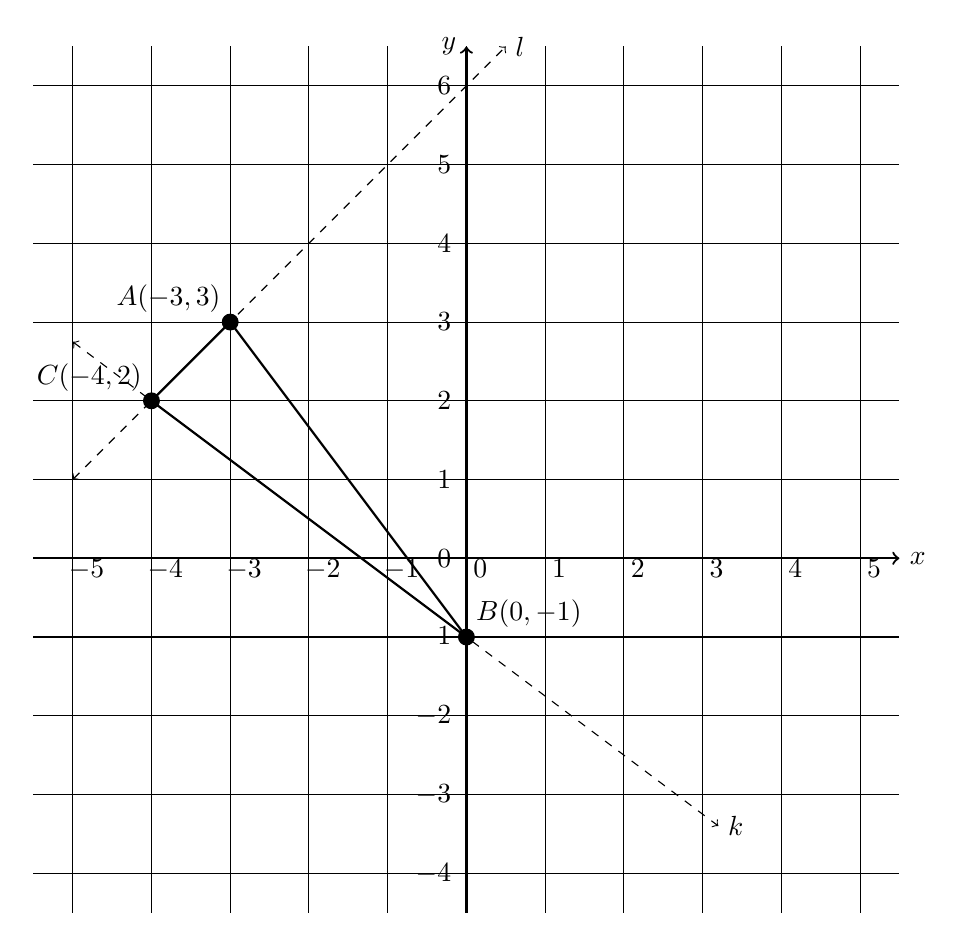
\begin{tikzpicture}[scale=1.0]
            %grid
                \draw [thin, color=black,, xstep=1.0cm,ystep=1.0cm] (-5.5,-4.5) grid (5.5,6.5);
                %\draw [thin, color=lightgray,, xstep=0.2cm,ystep=0.2cm] (-5.5,-4.5) grid (5.5,6.5);
                \foreach \x in {-5, -4, -3, -2, -1, 0,1,2,3,4,5}
                \draw[shift={(\x,0)},color=black] (0pt,-1pt) -- (0pt,3pt) node[below]  {$\quad \x$};
                \foreach \y in {-4, -3, -2,-1,0,1,2,3,4, 5, 6}
                \draw[shift={(0,\y)},color=black] (2pt,0pt) -- (-2pt,0pt) node[left]  {$\y$};
                \draw [thick, ->] (-5.5,0) -- (+5.5,0) node [right] {$x$};
                \draw [thick, ->] (0,-4.5) -- (0,6.5) node [left] {$y$};
            \draw [<->, dashed] plot[domain= -5:3.2] (\x, -0.75*\x -1)node[right]{$k$};
            \draw [thick] plot[domain= -4:0] (\x, -0.75*\x -1);
            \draw [<->, dashed] plot[domain= -5:0.5] (\x, \x +6)node[right]{$l$};
            \draw [thick] plot[domain= -4:-3] (\x, \x +6);
            \draw [thick] (-3,3)--(0,-1);
            \draw [fill] (-3,3) circle[radius=0.1] node[above left]{$A(-3,3)$};
            \draw [fill] (0,-1) circle[radius=0.1] node[above right]{$B(0,-1)$};
            \draw [fill] (-4,2) circle[radius=0.1] node[above left]{$C(-4,2)$};

        \end{tikzpicture}
        \end{center}



\end{enumerate}
\end{document}